\chapter{Computational Description}

% \Gls{homeostasis}
% \gls{glsy}

\section{Cognitive Systems}
\begin{quotation}
    \improvement[inline]{change size}
    \emph{What is a cognitive system?}
\end{quotation}

\subsection{The origin of cognition} \story{Discernment as the basic operator of cognition. What am I, what am I not. We want to show that the idea of the self is not clearly defined, but a dynamic process right from the beginning. We also show that a self needs to maintain a representation of itself and has the ability to hold counterfactual states.}

In [source: From Levin Talk on consciousness] Levin asserts that all agents have in common the ability to pursue goals and suggests that the size of the goal is a way to classify and compare diverse intelligences. For example, a single-celled organism may have the goal of finding food and avoiding predators, while a human may have the goal of building a family or writing a thesis about cognition.

Levin introduces the term \gls{cognitive light cone}, which metaphorically describes the limits of an agent's knowledge and ability to act. It is defined by the set of all events that an agent can perceive, measure, and model.

When thinking about the genesis of the self, we can think back to our earliest developmental stage, that of being an unfertilised \gls{oocyte}, \definition[inline]{oocyte (check exactly how it works. Does the sperm go in the oocyte? Is each sperm an individual or is each egg an individual? can there be multiple sperms in an oocyte? what are monozygotic, dizygotic, conjoined twins?)}, and realize that the self gradually emerges from it.

Levin shows that when scratching a \gls{blastoderm} \definition[inline]{blastoderm}, it self-organizes into twins or triplets, etc., depending on the amount of scratches. \source[inline]{source}. This demonstrates that the number of selves in an \gls{embryo} is not determined by genetics, but is instead a result of physiological self-organization. The problem of discerning between one's self and the external world is an ongoing, dynamic process that needs to be solved "online". This indicates that our self-concept is ever-evolving, reshaped by new information and experiences.

In \source[inline]{source} Levin expounds on the idea that the self-organisational process of bodies is fundamentally the same as that of minds. 
\improvement[inline]{not only in structure but in representation. i.e. can we show that the imagination, the conceptual world has the same structure as the actual hardware? is the software built by the same principle as the hardware? is it growing simultaneosly?}. 

All bodies are \emph{composed} of a multitude of levels of organisation, from single cells to entire organisms. Each tier of this hierarchy possesses unique competencies and goals, yet collaboratively works towards the organism's overarching objectives.

\Gls{embodiment} is the grounding of cognitive processes in bodily experiences. Bodies are not just passive vessels for minds but play an active role in cognition \source[inline]{Serge paper on embodiment, sensorimotor information}. 

Diving deeper into bodily self-organization, organisms such as axolotls exhibit a fascinating ability. Despite undergoing amputation, they can regenerate their limbs and halt precisely when restoration is complete. This ability, despite the variety of starting conditions and challenges, hints at an inherent bodily blueprint or internal representation. Intriguingly, this map is underpinned by bioelectrical patterns, which play a pivotal role not just in regeneration but also embryonic development.

Expanding on this, Levin notes that there is no marked distinction between neural and developmental tissue in this context. Both comprise ion channels and electrical synapses. In fact, novel techniques have emerged to both interpret and modify these bioelectrical blueprints. \source[inline]{source}

These "blueprints", or more precisely: endogenous bioelectric pre-patterns, guide the cells to arrange in a certain way and by manipulating them, for instance by introducing potassium ion channel RNA, Levin and his team successfully induced cells to form eyes in non-ocular locations. More impressively, in the absence of sufficient cells, the system recruits additional cells to realize this goal.

In one experiment, the team modified the bioelectrical pattern of a planarian to have a two-headed form. Upon injury, the planarian regenerated, aligning with this new, dual-headed pattern. This reveals, that the planarian is able to have a representation of a body state, different from its current state. It means it has a rewritable memory and is able to represent counterfactual states.

\improvement[inline]{
This may be a primitive precursor to symbolic thought. Perhaps even to visualization and imagination.
Perhaps moving from bioelectrical pattern representation of the brain, which is in a sense the first counterfactual, this may be the first primitive version of symbolic? representation, and allude to the brain being a machine to store more complex patterns. 
}

\subsection{Embodied cognition and circular causality: on the role of constitutive autonomy in the reciprocal coupling of perception and action}

\cite{vernon_embodied_2015}
In Varela's words, cognition is \textit{effective action}: action that preserves the agent's autonomy, maintaining the agent and its ontogeny, i.e., its continued development.

There are two hallmarks of a cognitive agent:
1. Prospection, i.e., prediction or anticipation
2. The ability to learn new knowledge by making sense of its interactions with the world around it and, in the process, enlarging its repertoire of effective actions.

Homeostasis refers to the maintenance of stable internal conditions within an organism, while allostasis refers to the adaptive regulation of these internal conditions in response to changing demands.

Both homeostasis and allostasis play a role in the reciprocal coupling of perception and action, as well as in the self-regulation of the agent's autonomy. (\gls{perception action cycle})

Autonomy is defined as the degree of self-determination of a system, i.e., the degree to which a system’s behavior is not determined by the environment and, thus, the degree to which a system determines its own goals. 

\rephrase[inline]{I would argue that the autonomy always depends on the levels above and below, in the hierarchy. i.e., we are part of a society, but we are also constituted of and encapsulated by simpler elements. Therefore we share the goals of those levels. Being part of an environment imposes an inductive bias.}

Living systems face two challenges: they are 

1. delicate: they are easily disrupted or destroyed by environmental forces, requiring avoidance or repair of disruptions.
2. dissipative: they are comprised of far-from-equilibrium processes, necessitating external energy sources to maintain their stability and avoid lapsing into thermodynamic equilibrium, which would threaten their autonomy or existence.

\info[inline]{relate (or reference) this to maxwells explanation of active inference.}

Cognition, is the property which helps look into the future, to avoid these problems.

There are two types of autonomy:

1. \emph{Behavioral autonomy} focusses on the external characteristics of the system: the extent to which the agent sets its own goals and its robustness and flexibility in dealing with an uncertain and possibly precarious environment.
2. \emph{Constitutive autonomy} focusses on the internal organization and the organizational processes that keep the system viable and maintain itself as an identifiable autonomous entity.

These two parts of autonomy enable each other recursively.

\info[inline]{this is again FEP, hoemeostasis, allostasis}

Operational closure refers to a system that is self-contained and parametrically coupled with its environment but not controlled by the environment. It is a characteristic of a system that maintains its autonomy by subordinating all changes to the maintenance of its organization. This concept is used to identify systems that are self-contained and exhibit self-production or self-construction.

Organizational closure, on the other hand, characterizes a system that exhibits self-production or self-construction and is recognized as a unity in the space where its processes exist. It is a necessary characteristic of autopoietic systems, which are self-organizing systems that self-produce and operate at the biochemical level. Organizational closure is related to the concept of constitutive autonomy, where a system actively generates and sustains its existence and systemic identity under precarious conditions.

Both operational closure and organizational closure are important concepts in understanding the autonomy and self-regulation of cognitive agents. They highlight the self-contained nature of these systems and their ability to maintain their organization and identity through self-production and self-construction processes.

Structural coupling refers to mutual pertubation of an agent and its environment.


\begin{itemize}
    \item Autopoiesis
    \item Heterarchy
\end{itemize}


Difference between self-organization and emergence:

Self-organization is a process where a global pattern emerges from numerous lower-level component interactions, while emergence refers to the generation of a global pattern that is qualitatively different from the assembly of components.

Self-organization is basically a macro-level structure out of smaller parts, emergence is when the whole is more than the sum of its parts.

Self-organization in emergence leads to systems with clear identities or behaviors due to local-to-global determination and global-to-local determination.

\info[inline]{relate this to piccininis distinctions of emergence. Also to michael levins observer dependent cognition (sth like that?) where function emerges by viewing the system in different ways.}

Autonomous systems are not only reactive but also preemptive and proactive, readying themselves for multiple contingencies and deploying strategies to deal with them while pursuing their defined goals. \info[inline]{we are not only reactive}
Such systems must therefore be able prepare for counterfactual states \info[inline]{link to counterfactuals}. 
Allostasis is concerned with adapting to change in order to achieve the goal of stability in the face of uncertain circumstances. \todo[inline]{link to hemispheres. apprehension vs ?}

Seth notes that "He notes that attention can then be viewed as a way of balancing active inference and model update, (referred to as precision weighting)."

\subsection{Active Inference} \story{Introducing the shared principle to build multi-scale systems. Essentially a formalization of discernment.}

\rephrase[inline]{From Maxwell Ramstead Tutorial on active inference}
    - The brain structure in a sense recapitulates the structure of its environment in which it is encapsulated
    (the paper Evidence of a predictive coding hierarchy in the human brain listening to speech is related to this)
- Paper by Park \& Friston shows nested networks: dendritic structure, neurons, brain regions, etc. 
- These multi-scale systems work in the spatial (microcosm to macrocosm) as well as in the temporal dimension (phylo-, epi-, ontogenetic)
- how would we address all these different spatial and temporal scales in a principled way what kind of framework would be able to enable
- Most self-organizing systems in nature tend to dissipate. (see vernon, section above)
- This means that they consume the gradients around which they organize. For example, a lightning bolt self-organizes around a charge gradient, and in striking, it consumes the gradient around which it's self-organized, effectively leaving the entire system at equilibrium. The same could be said for tornadoes, although in this case the gradient is temperature instead of charge.
- The main takeaway is that for almost all systems in nature, self-organization serves to increase entropy. In this context, entropy is a measure of spread. You can think about it roughly as a quantification of how many different configurations the system could be in. High entropy means a high number of available configurations, while low entropy means a low number of available configurations.
- roughly 80\% of the brain's connections are doing this feedback thing. they are descending so in a sense it would sort of be surprising that 80\% of the brain's energy budget goes to something that's just feedback
- How does meaning emerge from this? Somehow, meaning emerges from the aggregation of geometric features of stimuli. It's not clear how that's supposed to happen and we call this the *binding problem*
- The predictive processing view flips this on its head and says that maybe the brain is mainly engaged in top-down prediction. From this point of view, the main activity of the brain is to produce predictions about what it should expect to sense next. What flows up is the prediction error, which is the difference between what was predicted at a given moment and what is actually sensed.
- it's sort of like moving from a conception of the brain is a passive collector of data and a combiner of geometric or statistical information to a view of the brain as a kind of query machine.
- In the predictive processing view, perception is like a Google search. You ask a question and you get an answer. A visual cicada is as asking the world a question essentially, so perception is an answer to that question.
- Basically, the brain, according to active inference, is busy reversing this arrow. The arrow of causality goes from hidden States to data, and what we want to do is move from the data that we have to an inference of what the most likely causal factors are that caused the data.
- At layers above and at the same layer, any unit is receiving predictions about what it should sense. What's going on is a constant comparison between what the brain expects to perceive and what it actually does perceive, and the discrepancy between these two signals is what gets shuffled up the hierarchy.
- There are two ways to minimize this discrepancy:
	1. Change your model.
	2. Change the world.
- We have data and we're trying to infer the most probable latent States that cause the data that we're trying to explain. Causality flows in this direction, and inference flows in that direction.
- How can we quantify how well a model explains the data?
- The way that you typically do this is by constructing several alternative models that each encode a different hypothesis about how the data might have been caused. Then, you evaluate how well that model accounts for the variance in your data.
- If you want to compress this algorithm into a quantity, what you get is variational free energy. This is a measure of how much evidence is provided by the data for a given model of the process.
- It's important to stress that free energy is not the same as energy in the thermodynamic sense. It's a measure of how well your model explains the variance in your data.
- The reason it's called variational free energy is because it is analogous to the thermodynamic quantity free energy in thermodynamics, where free energy is the amount of energy left in a system that can perform work. In the information theoretic context the variational free energy is basically the amount of wiggle room you still have on your parameters.
- A Markov blanket is a way of saying that conditioned on the existence of a set of states, the sensory and active States of the system are independent of the external states of the world.
- Active inference then is a story about how internal states (which encode our model) and active States (which are like our skeletal muscles) change to minimize free energy, and the end effect is to allow this inference process to happen.
- All of the components of this system are also systems. This is the observation that we started with: I'm a system, I'm an organism, but I'm made of networks of organs that are themselves systems, and the organs themselves are systems of cells, and so forth.
- So every component of a Markov blanket is itself Markov blanketed. Cells that share a generative model and over time reach a target configuration. This is basically a little creature with a head and a tail. Everyone sees that, and so what you have plotted here is basically the beliefs of each cell about what kind of cell they are.
- They're able to infer their place relative to other cells so long as they're able to commute with other cells, because we all have the same expectations. We all expect to sense the same kinds of things.
- This is how you effectively connect levels of organization: units at one level sharing a generative model are able to enact a target morphology.

\subsection{Bioelectrical patterns and predictive processing} 

Bioelectrical patterns are generated by ion channels and electrical synapses, which are found in all cells, including neurons. These patterns can be used to control cell movement, differentiation, and communication.

In the brain, bioelectrical patterns are thought to play a role in a variety of cognitive functions, including perception, memory, and learning. For example, bioelectrical patterns in the visual cortex have been shown to correlate with the perception of visual stimuli.

The predictive processing view of cognition suggests that the brain uses top-down predictions to infer the causes of sensory input. These predictions are generated based on the brain's internal model of the world. The brain then compares its predictions to the actual sensory input it receives. If there is a discrepancy between the two, the brain updates its model of the world to reduce the error.

One way to think about the relationship between bioelectrical patterns and predictive processing is to consider how bioelectrical patterns may be used to generate predictions. For example, the bioelectrical patterns associated with a particular posture could be used to predict the visual input that would be received if the body were to move in a certain way.

The brain could then compare this prediction to the actual visual input it receives. If there is a discrepancy between the two, the brain could update its model of the world to account for the difference. This process of prediction and error correction could allow the brain to learn and adapt to its environment.

\subsection{Self-organization and predictive processing} \cite{friston_world_2021}
Self-organization is a process by which complex systems emerge from the interaction of simpler parts. The brain is a self-organizing system, and its predictive processing capabilities may have emerged from the self-organization of its neurons.

As the brain develops, its neurons self-organize into networks that are able to generate and test predictions about the world. This process of self-organization allows the brain to develop a model of the world that it can use to make inferences about sensory input.

One way to think about the relationship between self-organization and predictive processing is to consider how self-organization may allow the brain to develop a model of the world. As the brain develops, its neurons self-organize into networks that are able to represent different aspects of the world. For example, some networks may represent the visual world, while others may represent the auditory world or the somatosensory world.

These networks are constantly interacting with each other, and this interaction allows the brain to develop a unified model of the world. This model of the world can then be used to generate predictions about sensory input.

The identity of a multi-scale system can be thought of as the emergent properties that arise from the interactions of the different levels of organization. For example, the identity of a cell is not simply the sum of the identities of its individual molecules. Rather, the cell's identity is emergent from the way in which the molecules interact with each other to form complex structures and networks.

This is reminiscient of embedding spaces in which words are self-organizing by getting input from the world. 
\info[inline]{LLMs also create a generative model, but lack the causal structure.}

\todo[inline]{establish the argument for a generative model. Then we talk about the kind of generative model. Maybe introduce Transformers here already.}

\rephrase[inline]{From \cite{ciaunica_nested_2023}: “Self-organization is typically defined as the spontaneous emergence of spatiotemporal order or pattern-formation processes in physical and biological systems resulting from interactions of its components with the environment (Camazine et al. 2001; Seeley 2002, Rosas et al. 2018). Properties of a global higher level system emerge from—and are dependent upon—interactions of its components at the lower level. For example, when the wind blows over a uniform surface of sand, a pattern of regularly spaced ranges emerges (cf. FIG. 1) as a combination of gravity forces and wind speed act on the sand particles (Forrest and Haff 1992). In turn, the surface of the sand determines the flow of air, shaping the reports. Self-organisation therefore entails both bottom-up and top-down causation (Ellis et al., 2011) that is reflected in the circular”
“causality implicit in the enslaving principle (Haken \& Portugali, 2016) in synergetics or the centre manifold theorem in dynamical systems theory (Carr, 1981).”
“However, biological organization is more than emergent complexity. It is fundamentally composed of nested goal-seeking (homeostatic and allostatic) agents, ranging from molecular pathways to whole organ systems and beyond. These not only exhibit complex behaviour, but also specifically act to minimize and maximize various quantities and solve problems by navigating (with diverse degrees of competency) a variety of spaces including transcriptional, physiological, and anatomical spaces in addition to the familiar space of behaviour (Fields \& Levin, 2022).”}

\subsection{Identity and Essence}
Here we discuss homeostasis, allostasis | me against the world
\subsubsection{Categories}
\begin{itemize}
    \item Prototype Theory ( + prototype, stereotype, archetype) (types and relation to programming?)
    \item intension extension?
    \item LLMs
    \item mereology
    \item ontology
\end{itemize}

\begin{itemize}
    \item substance theory
    \item process theory
    \item krakauer information individuality
    \item Relationship between agent and environment. Embeddedness, we are inseperable; Üexküll called this bio-semiotics and the extended phenotype (the spiderweb is part of the spider, humans domesticated fruit, animals, etc. these are all part of what it means to be human.)
\end{itemize}

\subsubsection{Computational models of categorization}
Prototype models: These models represent categories as a prototype or central tendency of the features associated with a category. They assume that category membership is based on the similarity of an object to the prototype.
Exemplar models: These models represent categories as a set of stored examples or exemplars. They assume that category membership is based on the similarity of an object to the stored exemplars.
Feature-based models: These models represent categories as a set of defining features. They assume that category membership is based on the presence or absence of specific features.
Connectionist models: These models represent categories as patterns of activation in a neural network. They assume that category membership is based on the pattern of activation that results from processing sensory input.
Bayesian models: These models represent categories as a probability distribution over features. They assume that category membership is based on the likelihood that an object belongs to a particular category given its features.

What is the point here? what do I think? I think categories, similar to any self organizing system maintain a boundary of what they are and what they are not. they themselves can be thought as agents. We have the concepts but our perceptions are shaped ,mostly by evolution and society. Our subjective interpretation is actually minimal. Our perception of objects strengthens in concordance with the crowd, the society. So these concepts, which are sort of memes can be seen as agents themselves. They self-organise, and have a mapping to the actual underlying brain structure which is a mapping of the environment, to solve certain problems. a concept is the minimization or optimization of free variables in an active inference frame. This relates to gibsons affordances. so concepts might be formed also by function, or the relation of how i could interact with the concept. but concepts dont always have to be functional. this is also related to meaning. the function of a concept is its meaning. in that way it is the set of inferences one could make from said concept. of course it doesnt mean that it is meaningful, which is subjective to the observer and dependent on personal preference and goals. concepts are agents that serve a goal. notice how concepts have different levels of granularity, according to our interaction with them. 


\subsection{What is a thought?}
\begin{itemize}
    \item Explain the idea of a thought as a trajectory through semantic space. 
    \item How does this trajectory look like in LLMs? (Wolfram)
    \item How does this trajectory look like in GFlowNet? (perhaps operationalised as a Markovian trajectory?)
    \item How does a thought look like in enactivist/ purely reactive or reflexive cognitive frameworks. 
    \item Thought as constructing probabilistic programs
    \item What does it mean to have a model?
    \item What does it mean to compute?
    \item Can any concept be definitively defined as a particular concept (either symbolic or symbolic vector e.g. SPA, hyperdimensional vectors) or are all concepts approximations?
\end{itemize}

\subsection{What does it mean to understand?}
What does it mean to truly understand something? 

I would say that understanding requires causality, not just correlation. 

Is it possible for artificial intelligence to grasp the essence of a concept like “body” or “mass”? It can approximate to an arbitrary degree but you can't square the circle, i.e. approximations at the limit do not become the thing approximated, they are just treated as such. This is related to joscha bach's interpretation of Gödel's theorem, that it cannot be implemented since there are no infinities in physical reality. Anyways, approximations might be enough, and might be what we're doing too. This is important for the symbolic vs connectionist debate.

GPT learns through the context in which words and phrases appear, essentially creating a concept network of words. The AI analyses this abstract relational structure to generate responses. Yet, we might question whether this process equates to understanding.

The conundrum is reminiscent of the mary's room thought experiment, in which Mary, despite having all the data about colour, has never truly experienced it. If she were to experience colour one day, would she glean any new information that was not already available in the data she had studied?

The question seems to probe whether phenomenological experience can be simulated through abstract data. While it's possible to argue that a blind man will never truly see just by reading about it, we must also consider that our experiences are essentially the result of neurons firing in our brains. If we possess the necessary cognitive mechanisms, it's plausible that phenomenological experience could be replicated by alternative means.


\begin{itemize}
    \item are human's capabilities (or LLMs) just a bunch of bag of tricks, masquerading in a trenchcoat.
\end{itemize}

\subsection{Part-Whole Hierarchies/ Holarchies}
\begin{itemize}
    \item argue thoroughly why the conceptual framework is built as a holarchy
    \item We agree on an assumption that we construct a model of the world.
    \item What exactly would an explicit model or an implicit model or no model at all look like?
    \item We agree that there are certain hierarchical relationships. [example book, music, ontology, etc.]
    \item Here we can talk about conceptual structures, holarchy, part-whole hierarchies. 
    \item How concepts are split with more attention, etc. 
    \item Do the upper levels of a holarchy control the lower levels? I.e. Does the holarchy become a heterarchy?
    \item Heterarchy, sand example in nested organism pregnancy friston paper, DNA, GEB
    \item Multi-scale systems
    \item Ontology
    \item Mereology? and relation to Category theory?
    \item This is essentially learning a 
        \item hierarchical LVM
        \item hierarchical graphical model
        \item Parse tree
        \item Can be formalised as Context Free Grammar. 
        \item The grammar here is the generative model. 
        \item What is a generative model?
        \item A generative model is simply a probabilistic description of how causes (i.e., latent states) generate consequences (i.e., data or sensations). \cite{friston_world_2021}
    \item Include Hofstader levels of abstraction (let's have a coffee.)
\end{itemize}

\improvement[inline]{Shared competencies, or similar strategy between compositional hierarchical structures in organisms and in the construction of concepts/ thoughts}

\rephrase[inline]{From "Building machines that learn and think like people}
Compositionality pertains to the formation of new representations through the combination of simpler, primitive elements \cite{Lake_Ullman_Tenenbaum_Gershman_2017}.

Compositionality is central to cognitive productivity and learning. It allows for the creation of infinitely varied representations from a finite set of basic elements, similar to the mind's capacity to think an endless array of thoughts or generate countless sentences. This is particularly useful in forming hierarchical structures that simplify complex relationships, thus making inductive reasoning more efficient.


\subsection{Correlation Does Not Imply Causation}

Generative models assign probability distributions, representing observations in such a way that they can generate new data points similar to the observations. The mapping between the probability distributions and the data is correlational. They can therefore be described as \textit{correlational models}.
Causal models in contrast, represent hypotheses of how observations were generated. They do not just represent the observations by correlation, but aim to accurately reflect the mechanisms by  which the data originated.[source]
Significant challenges persist in deducing latent causal variables. [source]

Another crucial aspect of human cognition is the ability to acquire new knowledge and skills more quickly and easily by leveraging prior knowledge and experience. We can decompose situations quickly into basic components, e.g. when approximately understanding the anatomical composition of humans, we can quickly find the essence and apply it to mammals. We can parse scenes and situations into parts and generalize to other circumstances. 
This is related to surfaces and essences. 
Similarly to organisms which are composed in a nested hierarchy, each level of the nested hierarchy solves problems in their own domain without the need to being micromanaged from the level above, i.e. the process of self organisation happens at each level independently, so similarity it is crucial that learning to learn happens at multiple levels of the holarchy. 
For example, a machine that learns a compositional representation of a car can understand that a car is made up of parts such as wheels, an engine, and a chassis. This knowledge can then be used to learn new things about cars, such as how to drive a car or how to fix a car.

Using GFlowNet we can make inferences about intermediate variables. This is because we approximate probability distributions and not point estimates.


\info[inline]{argument for having two systems 1, 2}
\subsection{Thinking fast}
\cite{Lake_Ullman_Tenenbaum_Gershman_2017}
"4.3. Thinking Fast The previous section focused on learning rich models from sparse data and proposed ingredients for achieving these human-like learning abilities. These cognitive abilities are even more striking when considering the speed of perception and thought: the amount of time required to understand a scene, think a thought, or choose an action. In general, richer and more structured models require more complex and slower inference algorithms, similar to how complex models require more data, making the speed of perception and thought all the more remarkable. The combination of rich models with efficient inference suggests another way psychology and neuroscience may usefully inform AI. It also suggests an additional way to build on the successes of deep learning, where efficient inference and scalable learning are important strengths of the approach. This section discusses possible paths toward resolving the conflict between fast inference and structured representations, including Helmholtz machine–style approximate inference in generative models (Dayan et al. 1995; Hinton et al. 1995) and cooperation between model-free and model-based reinforcement learning systems."

\begin{itemize}
    \item Efficient inference over hierarchical Bayesian models is still difficult.
    \item Approximate inference
    \item Here we can go into models monte carlo e.g. etc.
    \item Einstein: intuition, rationality
    \item 
\end{itemize}


\info[inline]{argument for hemispheric lateralization}
\begin{itemize}
    \item Broad vs narrow attention. One sees the trees, the other the forest.
    \item the left wants to jump to conclusions and is much more quick and dirty, while the right says hang on
    \item left deals with things that are known, when something isn’t, its better to leave it to the right until it can be categorised by the left
    \item things in the left are more isolated, while in the right everything is connected to everything else
    \item left is static, right is flowing and changing
    \item the left abstracts, the left is more interested in categories, the right in the unique case
    \item the left sees things as inanimate, the right sees them as animate
    \item as we age we use the representations of what we know increasingly, neglecting the world. We become more solipsistic. This makes sense because perceiving things for the first time is computationally heavy and expensive, so the things we know from experience will usually be good enough.
\end{itemize}

Often, the most obvious things, once unpacked, reveal the most [examples?]. Our most basic perceptions and assumptions are so deeply integrated into our cognitive processes that they become invisible to us, essentially automatic. When driving the same route everyday, people may arrive at their destination without conscious awareness of it. Tasks become automated. [show studies, other examples like piano.]

From a computational standpoint, one could say that these deeply embedded perceptions function much like 'compiled code' in a computer program — efficient and fast, but not easily inspected or altered. These perceptions are model-based representations optimized for computational efficiency, trading off flexibility for speed. They exist as pre-computed "shortcuts" that enable us to interact with the world without incurring high computational costs each time we encounter a familiar situation.

In machine learning, this relates to the trade-off between model-based and model-free learning. Model-free approaches require higher computational costs upfront but are more adaptable. Model-based strategies offer efficient but rigid ways to interact with the world. Both strategies have their pros and cons, reflecting a trade-off between computational efficiency and cognitive flexibility. [source]

As we age, we rely increasingly on these internal representations instead of engaging directly with external reality, making our view of the world more solipsistic. [source]

This phenomenon can be explained by the increasing reliance on "cached" or "memoized" cognitive models, which offer a computationally cheaper way to navigate reality. It's a form of cognitive "greedy algorithm," opting for local optimizations based on past experience rather than recalculating the optimal path each time. [source + relation to predictive coding paradigm]

This concept parallels the notion of "overfitting" in machine learning, where a model becomes so tailored to the training data that it loses generalizability. In human cognition, an over-reliance on established mental models could result in decreased adaptability and an insular worldview, effectively isolating the individual from the ever-changing external environment.

As we automate more cognitive functions—either through learned habits or technological aids—we engage less in "active sampling" of the world, reducing the richness and nuance in our perceptions. This leads to a form of "lossy compression" of reality, where only the most salient features, according to our models, are retained.


- Problems should be solved at the lowest possible level of the hierarchy. Larger goals require more sophisticated organization.
- How does a system recognize that it cannot solve it alone and that it needs to recruit other cells? Think of the computational boundary. Perhaps we must be able to estimate computational complexity. 
- This compression of sensory information into concepts may be the origin of symbolic processing. 

- Things we don't have concepts for don't exist. We can't describe them in our language. [related to joscha about truth.] 


% \subsection{}

% Introduce Transformer architecture and 

\subsection{From Language to Consciousness: JB (Check Craft note)}
- Concepts are the address space of mental representations. They are merely pointers. 
- There's a hierarchy (holarchy) of abstraction of mental representations
- The least abstract thing are impulses that come from sensory neurons. 
- Basically, discernible difference, which is how we define information, is the closest to physical reality.
- We organize them into features. features describe how reality changes in the aggregate from moment to moment.
- Features are arranged into objects
- Objects remain stable if the perspective changes
- Concepts abstract over all objects that belong to a group - the extension of a category
- These concepts are organized in an embedding space

Conceptual space (relate this to Gordenford)
\begin{itemize}
    \item relationship path 
    \item mutual information (how well do concepts predict each other, co-occurence in reality)
    \item change distance
    \item parameter distance (related to hofstadter mathemagical themas)
\end{itemize}

Meaning: You establish the relationship between pattern and the function that describes the universe, your conceptual model, and that is meaning. Meaning is your entire mental universe. It's the unified model of reality that your mind is constructing. So for any new thing, if we can establish a relationship between the thing and our model, it has meaning. If we can place it in our conceptual framework, it gets meaning. 

\improvement[inline]{difference between what is meaning and what is meaningful, maps of meaning. what is meaningful is what guides you. its a gradient, a heuristic. Show studies that deeper understanding improves memory and meaning.}

\subsection{Free-Energy Principle}
\begin{itemize}
    \item Discernment of Concepts
    \item Discernment as the primary operator. 
    \item Me against the World
    \item Homeostasis
    \item Allostasis
    \item Operational Closure
    \item Organizational Closure
    \item Intentional Stance
    \item Active inference
    \item Explain Bayes theorem and how it relates 
\end{itemize}

\begin{equation}
    \underbrace{F(s, \mu)}_{\text{Free Energy}} = \underbrace{D_{KL}\left(q(\psi|\mu) || p(\psi|a)\right)}_{\text{Complexity}} - \underbrace{E_q\left[\log p(s|\psi, a)\right]}_{\text{Accuracy}}
\end{equation}

where the complexity is the Kullback-Leibler divergence between the true posterior and its approximation. The Accuracy is essentially the expected negative log likelihood (?)  

The FEP states that systems minimize their free energy by updating their internal models and taking actions that are consistent with those models. This can be done by:

Updating the internal model: Systems can update their internal models based on sensory feedback. This is done by comparing the predicted sensory input to the actual sensory input and adjusting the internal model accordingly.
Taking actions: Systems can also minimize their free energy by taking actions that are consistent with their internal models. This is because actions that are consistent with the internal model are more likely to lead to sensory input that is consistent with the internal model.

\cite{friston_world_2021}
Crucially, free energy is a functional (i.e., a function of a function) of two quantities. First, sensory data and a probability distribution over the unobservable states generating those data. This variational density is taken to be encoded, represented, or parameterised by the internal states of any system, ranging from a particle to a person. On this view, perception corresponds to changing internal states to minimise the divergence between the variational density and the posterior density over latent states, given observations. Conversely, action can change the way that data or sensations are sampled—to ensure that they provide the greatest evidence for the generative model entailed by an agent. This dual aspect—to optimising free energy—gracefully accounts for action and perception, where both are in the service of maximising (a variational bound on) marginal likelihood. 
In general, there are three levels of optimisation under the free energy principle. These correspond to the unknowns (i.e., latent causes) in the generative model. These unknowns comprise (i) latent states generating outcomes, (ii) model parameters encoding contingencies and statistical regularities and, finally (iii) the form or structure of the generative model. Each is equipped with variational density (i.e., a Bayesian belief) that is parameterised by the (i) states, (ii) weights, and (iii) structure of the agent at hand.
At the fastest timescale, inference can then be read as optimising the states (e.g., synaptic activity) to optimise variational free energy. This is usually cast in terms of a gradient flow on free energy. Crucially, the gradients of free energy can almost universally be cast as prediction errors.
The second set of unknowns are the parameters of the generative model, encoded in slowly changing weights (e.g., synaptic efficacy).Finally, we have the structure or form of the model, e.g., cortical hierarchies in the brain (Mumford, 1992). The structure of the model can be regarded as being optimised with respect to free energy or model evidence via a process of Bayesian model selection; namely, selecting those models with the greatest marginal likelihood, as assessed over an extended period of time. This level of optimisation manifests at different scales. For example, one can construe natural selection as nature’s way of performing “Bayesian model selection—i.e., accumulating evidence about an econiche by selecting phenotypes that have high adaptive fitness or marginal likelihood (Campbell, 2016; Frank, 2012). At a somatic timescale, in biology, this could be regarded as neurodevelopment with (epigenetic) hyperpriors over model structure. In cognitive science, this kind of optimisation process is often referred to as structure learning”
Above, we divided optimisation into inference, learning and model selection. However, a finer grained analysis of inference calls for a consideration of the representation of uncertainty. If one subscribes to the free energy principle, then optimisation corresponds to optimising posterior or Bayesian beliefs (or their sufficient statistics). This means that it is not sufficient to use point estimates of various quantities, the precision or inverse dispersion (i.e., negentropy) of these beliefs also has to be optimised. Sometimes this is a more difficult problem that estimating the average or expectation of an unknown \rephrase[inline]{here he says that point estimates are not enough. so MLE over MAP}
\improvement[inline]{this relates to gflownets representing the posterior}
- log model evidence can be decomposed into accuracy and complexity. The complexity of a generative model corresponds to the kullback leibler divergence between posterior and prior. in other words the effective number of parameters or degrees of freedom that are required to accurately account for some data and its sampling. “Optimising free energy, therefore, puts pressure on finding the simplest explanations and models” 
This is exactly the same idea that underwrites the minimisation of algorithmic complexity in the setting of minimum description or message length schemes
discrete actions solicit a sensory outcome that informs approximate posterior beliefs about hidden or external states of the world – via minimisation of variational free energy under a set of plausible policies (i.e., perceptual inference). The approximate posterior beliefs are then used to evaluate expected free energy and subsequent beliefs about action (i.e., policy selection). Note a subtle but important move in this construction: the expected free energy furnishes prior beliefs about policies.
it means that agents infer policies and, implicitly, active states. In other words, beliefs about policies – encoded by internal states – are distinct from the active states of the agent’s Markov blanket. In more sophisticated schemes, agents infer hidden states under plausible policies with a generative model based on a Markov decision process. This means the agent predicts how it will behave and then verifies those predictions based on sensory samples. In other words, agents garner evidence for their own behaviour and actively self-evidence.
Another technological idea is the 'game engine in the head', i.e., the use of very fast approximate simulators for graphics physics and planning, which can simulate complex physical situations in realistic ways and use those as a prototype for the model in the agent’s head. It is something like an approximat ion to the common-sense systems of understanding the world, that evolution has built into our brains, and that even young babies can use to explore the world.


\begin{itemize}
    \item I guess in simple terms, it means that internal states are being updated or refined, whenever they are incongruent to the observations.
\end{itemize}


\cite{mazzaglia_free_2022}
“The free energy principle originated from the work of von Helmholtz on ‘unconscious inference’ [57], postulating that humans inevitably perform inference in order to perform perception. This implies that the human perceptual system continuously adjusts beliefs about the hidden states of the world in an unconscious way.” ([Mazzaglia et al., 2022, p. 3]

“According to the free energy principle, in order to minimize free energy, the agent learns an internal model of potential states of the environment.”
“Crucially, these internal states do not need to be isomorphic to the external ones, as their purpose is explaining sensorial states in accordance with active states, rather than replicating the exact dynamics of the environment. Isomorphism, in this context, refers to considering a structure-preserving mapping of the state space.”

Because of these assumptions, the concept of 'reward' in active inference is very different from rewards in RL, as rewards are not signals used to attract trajectories, but rather sensory states that the agents aims to frequently visit in order to minimize its free energy

Training the model is then typically alternated with collecting new data by interacting with the environment, using the model for planning [49], or using an amortized (habitual) policy [67, 33]. In practice, one can also train a model upfront using a dataset of collected trajectories from a random agent [68] or an expert [32]. The latter is especially relevant in contexts where collecting experience online with the agent can be expensive or unsafe [69].


\subsection{generative models}
% \section{Spaces in Cognition}
% \subsection{Latent Spaces}
% \subsection{Cognitive and Conceptual Spaces}
% \subsubsection{Peter Gärdenfors's Perspective}
% \subsection{The Geometry of Cognitive Spaces}
% \subsubsection{Hyperbolic Spaces}

\begin{itemize}
    \item show representations in human brains and argue why the brain may largely be a generative model. 
\end{itemize}



\subsection{hierarchical generative model}
\begin{itemize}
    \item amortized sampling tutorial
\end{itemize}

\subsection{Organisms across scale and multi-scale cognition}

\begin{itemize}
    \item Cellular Automata
    \item Lenia
    \item (Pure) Enactivism?
\end{itemize}

\subsection{Language in Thought}
\begin{itemize}
    \item Syntax \& Semantix
    \item Jabberwocky sentences (would be equivalent to a sentence that doesn't minimize surprise well (given the task, because it could also be a goal))
\end{itemize}

\begin{itemize}
    \item Sapir-Whorf
    \item Why do we need language
    \item Does meaning emerge in LLMs (is meaning the network or do we need grounding)
    \item Grounding
    \item Binding problem
\end{itemize}

\subsection{LLMs}
\begin{itemize}
    \item Self-Attention
    \item Successes
    \item Limitations
    \item relation to part-whole hierarchies, FEP, grounding, etc. 
\end{itemize}

\subsubsection{Limitations}
\rephrase[inline]{from JB: LLMs learn how to complete sequences, they do statistics over patterns
patterns → syntax → style → semantics
they deep-fake so well that the outcome becomes indistinguishable from what we do. thats why its said to brute force. 
Minds learn how to understand
we do it the other way around
semantics → patterns → syntax → style}

\subsection{Human's capabilities}
Humans naturally exhibit the aptitude to innately evaluate the reliability of our knowledge. Understanding the limits of one's knowledge directs the acquisition of new information, thus optimizing the learning process.

Moreover, human cognition is characterized by modularity and reusability. Our mental architectures are adept at disentangling knowledge into modular components, which can be recalled, combined, and repurposed to address novel challenges.
By continuously crafting and refining abstract concepts, humans can process, assimilate, and communicate multifaceted knowledge structures with remarkable efficiency.

Further, we intuitively discern causal relationships, allowing for predictive and counterfactual reasoning.
Causal models, seen as extensive distribution families influenced by interventions, provide the scaffolding for this intuitive understanding. As highlighted by Kemp et al. (2015), these models enable humans to extrapolate beyond observed data, envisage hypothetical scenarios, and navigate the world with a goal-oriented mindset. In computational terms, integrating causality can tremendously amplify the generalization capabilities of algorithms, allowing them to predict outcomes under novel interventions and facilitating deeper understanding of intricate systems.

Often there are multiple solutions to a query, which is why the inference network should model a multimodal distribution rather than a point estimate. Difference between MAP and MLE. 

\begin{itemize}
    \item Throw in some definitions for intelligence. (+ Analogy)
    \item Out-of distribution data, imagination, simulation
    \item Types of questions [check note: categorizing questions] (equivalent to inference types?)
\end{itemize} 

\subsubsection{Operationalising "Understanding"}
\begin{itemize}
    \item Reverse Engineering: Is understanding being able to reconstruct the thing we want to understand? If you can break down an object or concept and then reconstruct it, perhaps it implies you understand it.
    \item Modelling: Understanding might be proportional to the model we create of a concept. The more accurate and comprehensive our model, the greater our understanding.
    \item Utilization: It could also be the degree to which we can use a concept. If we can apply it effectively, we could claim to understand it.
    \item Maybe understanding is the size/ strength of a concept? Imagine it as blobs in an abstract space, a large blob with many connections would be understood, whereas a new little blob with little connections is not. 
\end{itemize}

\begin{itemize}
    \item Children use language without knowing what the words actually mean. The meaning is the context. 
    \item People can even teach without understanding. 
    \item Fake it 'til you make it?
    \item Is the limit of imitation a clone? ()
\end{itemize}

\subsection{System 1 and 2}

\begin{itemize}
    \item Slow, Fast
    \item Reflexive vs Reasoning (reflexive is the direct response of the generative model, while reasoning is a higher level model, essentially a model over the reflexive part (this is also why we are not conscious over reflexive actions. Think e.g. how we don't notice driving a familiar road))
    \item Transformers are correlational, we need to build causation. this is the same as reflexive vs reasoning.
    \item does, or when does, correlation approximate causation? Are humans correletional (reflexive but really complex) or causal? Wouldn't causality mean that we have free will?
\end{itemize}

\subsubsection{Poverty of the Stimulus}
The "poverty of the stimulus" argument is an argument that is often made in the field of linguistics and cognitive science. It argues that children are able to learn language despite being exposed to a relatively limited amount of data, which suggests that they must have some innate knowledge or ability that helps them learn language.

The argument is based on the observation that the linguistic input that children receive is often incomplete, ambiguous, or inconsistent. For example, children may hear sentences that contain errors or that are not grammatical. Despite this, children are able to learn the rules of their language and use them to produce and understand sentences that they have never heard before.

One possible explanation for this is that children have innate knowledge or abilities that help them learn language. For example, it has been proposed that children have an innate knowledge of universal grammar, which is a set of grammatical principles that are common to all human languages. This knowledge enables children to quickly learn the rules of their language, even when the input they receive is incomplete or ambiguous.

The poverty of the stimulus argument is controversial, and it has been challenged by some researchers who argue that children are able to learn language by relying on general cognitive abilities, such as statistical learning or pattern recognition. However, the argument continues to be an important topic of debate in the field of linguistics and cognitive science.

\subsection{Hemispheric Lateralisation}
\begin{itemize}
    \item notion that if we don't have a concept for it, it does not exist for us. I.e. even if our sensory equipment can in principle take it in, and does take it in, it is not there for us. It seems we are unable to attend to it. Perhaps attribute meaning to it and therefore it doesn't enter our conscious awareness.
\end{itemize}

\subsection{Language of Thought}

One of the most fascinating undertakings of Artificial Intelligence (AI) is its objective to reveal and learn from the mechanisms of human cognition.
--
The idea that the thoughts are constructed by some kind of Language of Thought (LOT), in order to understand and represent our reality has a long history. 
Gottfried Leibniz imagined a \textit{Characteristica Universalis}, a formal language capable of expressing metaphysical concepts \cite{sep-leibniz-logic-influence}.
Jerry Fodor, among many other scholars, developed this hypothesis, and proposed that thoughts are composed according to some form of internal grammar \cite{sep-language-thought}.
If our thoughts are indeed composed by some language, we can let our intuitions about its structure and limitations be guided by the advances made in the past century in regards to formal languages and computationalism.
Gödel showed that any formal system strong enough to express Peano Arithmetic is incomplete \cite{sep-goedel-incompleteness}. Turing showed that any possible computation can be done by a Turing machine and concluded that the human mind must be computational \cite{JCopeland2004-JCOTET}. [Piccinini disagrees]
Chomsky's Hierarchy classifies formal languages of different strengths and the automata that recognize them \cite{chomsky1959certain}.
These results and many more are consequential when thinking about a language of thought.
Many important questions about concepts are still left unanswered, e.g. regarding their formation, the structure of the framework they reside in, their representation, how they connect to other concepts and so on. 
Many contemporary versions of the LOT hypothesis (LOTH) argue that our conceptual framework is constructed bottom-up using some initial primitives. More so, the language we construct concepts in is executable, akin to a programming language \cite{dehaene_symbols_2022}. The idea is that we model the world by creating programs that generate our observations \cite{rule_child_2020}. 
Roumi et al.'s experiment indeed suggest that humans may interpret and compress sequence regularities in a type of program of minimum description length (MDL) \cite{al_roumi_mental_2021}.
Dehaene et al. further test this hypothesis and find similar results \cite{dehaene_symbols_2022}.
The question then remains, where primitives actually come from.
Piantadosi asserts that symbols have no inherent meaning, instead, meaning emerges from the dynamic relations between symbols. I.e., only the conceptual role and the dynamics of the symbols define meaning \cite{piantadosi2021computational}.
By defining meaning as an emergent phenomenon of conceptual roles, Piantadosi and Hill do not rule out that large language models (LLM) already have some foundation of meaningful concepts \cite{piantasodi2022meaning}.
Recent work tries to relate these ideas to biological systems, e.g. Quan et al. propose how role-filler interactions could be implemented in the brain via temporal synchrony to permit symbolic processing and dynamic binding of variables \cite{do2021neural}.
Santoro et al. argue for a semiotic approach, assert that symbols are subjective, and propose that meaning of symbols in artificial systems will arise when they are subjected to socio-cultural interactions \cite{santoro2021symbolic}.

Ellis et al. use $\lambda$-calculus, which is Turing complete, to build something akin to a LOT \cite{ellis_dreamcoder_2021}. In response, Piantadosi shows that combinatorial logic is equivalent to $\lambda$-calculus and why combinatorial-logic-like (LCL) language is preferable, for one because it doesn't assume primitives, thereby avoiding the problem of their meaning and origin. 
One of the questions regarding a LOT is whether thoughts can be produced by simple syntactic symbol manipulation.
I (and many others) suspect that semantics are not just an emergent phenomenon but that it actively shapes our perception and concept formation \cite{santoro2021symbolic, hofstadter_gdel_1979}.
Moreover, purely symbolic attempts, albeit being the original approach of artificial intelligence, have proven to be insufficient \cite{garcez2020neurosymbolic}. Instead, the successes of modern AI are owed to the advances of connectionist models. These however, have their own deficits, namely, being incredibly data-hungry, lacking causality, and lacking out-of-distribution generalization, to name a few. Therefore, new approaches try to combine these two AI strands into what is known as \emph{neurosymbolic AI} \cite{garcez2020neurosymbolic}.




\begin{itemize}
    \item What is the LOT in relation to the generative model?
    \item Is the LOT the policy over the gen model?
    \item do we need them to be distinct? (PCFG vs Q), Bengio
    \item Relation to self-organization, active inference, FEP, autopoiesis, etc. 
    \item show JBs argument of LLMs learning from 
    \item From Donald hoffmann and joscha bach: consciousness , etc. .. : proof cannot reach truth. godel found that there is truth that cannot be found with mathematics. but the opposite is true. there is no deeper notion of truth than proof. perception cannot be true or false. it just is. physical events cannot be true or false, a pattern you observe isnt true or false. the pattern itself is an interpretation. its hermeneutics. in order for something to be true or false you need a language which needs to be defined such that truth can be established. And the process of establishing truth is a computation. There are two types of languages in which truth can be defined: classical mathematics is stateless and thus timeless. it lacks the temporal dimension. this allows you to create functions that take infinitely many args in a single step. but in a computational system you cannot assign a single digit to pi. here, in a language with steps, we are losing the ability to treat pi as a value. it is now a function we can only approximate to a certain degree. we get a fundamental difference between a value and a function. (relate this to the universal function approximator: can we approximate downstream functions? perhaps thats what we need symbols, or grounding for). this means that also truth changes. its no longer this platonic thing that exceeds mathematics . it has to be contingent on the language that uses it. if the language has internal contradictions, truth becomes impossible to determine and you can never prove statements that cannot be described in your language (extrapolation). 

    In essence it means that we can define languages which do not align with the real world, but are above it. we need to define languages of the same level as actual reality. 
    \item what is a symbol and what is a symbolic architecture. symbolic here literally means symbol manipulation. context free grammar, etc. logical predicates. DC makes it neurosymbolic by using nns. I make it even more connectionist by embedding the symbols.
    \item Explain the different gradients of symbols. e.g. SPA is symbol-like. Part whole hierarchies and capsules are also kind of a symbol in that there is a central representation of a concept. I think its about centrality vs distributed representation and also about the capabilities of the symbols, i.e. does cognition work by only manipulating the symbols, rather that the representations themselves? What is that extra layer needed for then? Think of SPAs layered vectors, shallow vs deep understanding.  
\end{itemize}

Free will: if i can out model you, i.e.  i can predict every action you do, 


\subsubsection{Neurosymbolic AI}
\rephrase[inline]{Our conclusion from the above discussion is that in neurosymbolic AI: • Knowledge should be grounded onto vector representations for efficient learning from data based on message passing in neural networks as an efficient computational model. • Symbols should become available as a result of querying and knowledge extraction from trained networks, and offer a rich description language at an adequate level of abstraction, enabling infinite uses of finite means, but also compositional discrete reasoning at the symbolic level allowing for extrapolation beyond the data distribution. • The combination of learning and reasoning should offer an important alternative to the problem of combinatorial reasoning by learning to reduce the number of effective combinations, thus producing simpler symbolic descriptions as part of the neurosymbolic cycle. \cite{garcez_neurosymbolic_2020}}

\subsubsection{Formal Grammar}
\begin{itemize}
    \item Syntax vs. Semantix
    \item Semiotics
\end{itemize}

% \subsection{Gödel's Incompleteness Theorem and Turing's Extensions}
% \subsection{Chomsky's Hierarchy}
% \subsection{Computational Irreducibility}
% \subsection{Constructivism}
% \subsection{Syntax vs. Semantics in Language}
% \subsection{Semiotics}
% \subsection{The Notion of a Semantic Grammar}
% Church-Turing Thesis


\subsection{Computational Mind}
\begin{itemize}
    \item RNA computation
    \item Church-Turing Thesis
    \item Difference in computation between brain (Piccinini), ANNs and symbolic processing
\end{itemize}

\subsection{Some approaches}

\begin{itemize}
    \item GLOM also related to NCA and to holarchies
    \item Kissner
    \item JEPA
    \item etc. 
\end{itemize}




Constructing compositional structures

\subsection{Compositional world model and inference machine}

In a language of thought, we make the assumption that thoughts are compositional. In one way or another, thoughts are hierarchical (?).
Both in ontologies, i.e. the way concepts are structured, (animal - bird - fink) but also in the sequential nature of thought construction (as in natural language, reasoning tasks, etc.). We are creating parse trees, or abstract syntax trees. 

\begin{itemize}
    \item but there is a difference between ontology, i.e. the structure of all concepts vs the sequential construction of thoughts.
    \item so what are we simulating here?
    \item One is the generative model. the world model. the other is the inference machine. 
\end{itemize}

It seems that we have essentially two problems 
\begin{enumerate}
    \item Constructing a conceptual framework, with relationships of all concepts.
    \item Navigating this conceptual framework. 
    \item maybe the generative model is correlational, while the inference model turns that into causality. (see beyond the fep internalism externalism, ramstead)
    \item I think having a sense of self, i.e. a self-referential story, involves this inference model that builds causal structure, a narrative (see \cite{bouizegarene_narrative_2020}).
    \item Is this related to interpolation vs extrapolation? (is it the same in high dimensions? chollet?lecun?)
\end{enumerate}

We want to find out

\begin{enumerate}
    \item Where the self emerges.
    \item What is meaning and what is meaningful
\end{enumerate}


\begin{itemize}
    \item Do we have one generative model or multiple competing models? Or do we just have competing representations at the frontier and it is more difficult to change beliefs deeper in the conceptual space, where concepts are foundational and others rely on?
    \item Jerome Busemeyer uses Quantum formulations to show how we are in a super-position of beliefs until we collapse them upon evidence. 
\end{itemize}

The renowned professor Yoshua Bengio explains that thoughts are composed of multiple intermediate steps and explains that reasoning, or thinking, is the combination of knowledge and inference. 
He theorises that we construct a world model which may take the form of an energy based model.

It is interesting to think about whether this world model is explicit or implicit. In DreamCoder and other SOTA methods in program synthesis the world model is essentially an explicit PCFG from which one samples programs. In neural program synthesis, the new approach of neurosymbolic programming, the role of the neural network is to act as a recognition model, helping to search programs from this PCFG.
I imagine it a little different, and see the thought construction process more like an agent, following a policy.

On one side, in alignment with Occam's razor, our world model aims to identify the essential knowledge fragments required to interpret observed data. This model should be concise, optimizing the encoding bits and enhancing the reutilization of knowledge segments, thereby enhancing its generalization capability to unfamiliar scenarios. This aligns with the principle of parsimoniousness or, as Dehaene describes as finding programs of minimum description length.

A trained inference machine amortizes the cost of searching through a vast solution space which resource-intensive search methods like MCMC, traditional AI techniques, or optimization algorithms cannot handle.
In conclusion, approximate inference could be the solution here, since a larger model doesn't lead to overfitting but better approximations, while not being dependent on lots of data.

Yoshua warns that a notable vulnerability of current large language models is the conflation of the world model with the inference mechanism. Although LLMs may construct an implicit world model, the distinction between world model and inference may be the underlying cause of their difficulty for out-of-distribution prediction \cite{goyal_inductive_2022, yoshuabengioScalingService}.

\begin{itemize}
    \item RL
    \item MCMC
    \item variational inference
    \item amortized variational inference
\end{itemize}

\begin{itemize}
    \item the transcendentals as the axioms of ontology
    \item proto-concepts
    \item concepts vs no concepts
    \item concepts as pointers
    \item normalizing over sensory data -> features -> objects -> concepts 
    \item Concepts could be "chunked" into hyperdimensional vectors
\end{itemize}

\subsection{Problem Statement}
How do parts combine to solve shared goals?

\info[inline]{Formalizing the problem as constructing thoughts out of concepts in a vast state space. This is the general notion of building thoughts out of more primitive components. We don't define the nature of these components here. They could be programs or hyperdimensional vectors, or other stuff.}

\begin{itemize}
    \item Combinatorial search problem in which compositional latent hierarchical variables need to be found
    \item Amortized inference/ sampling
    \item GFlowNet?
    \item We want to show that the overall objective is to learn a model that samples proportionally to a given reward distribution
    \item Formalise the GFN approach
    \item Talk about induction, deduction, abduction and how sampling from a reward distribution is similar to abduction aka inference to the best explanation
    \item add markpoels 7 criteria 
\end{itemize}


\chapter{Implementational Description}


\section{Program Synthesis}

\subsubsection{CFG}

1. Background and Introduction

The field of programming has always been underpinned by the intricacies of formal grammars. Context-Free Grammars (CFGs), a subset of formal grammar, are essential in defining the syntactical structures of many programming languages. However, given the generative nature of CFGs, the potential program space defined by even a modestly complex grammar can be immensely vast. Searching for a specific program within this space, or ensuring that a particular space is sufficiently explored, poses significant computational challenges.

2. Problem Definition

2.1 CFG and Program Space

Let \( G = (N, \Sigma, P, S) \) be a Context-Free Grammar, where:
\begin{itemize}
    \item \( N \) is a finite set of non-terminal symbols.
    \item \( \Sigma \) is a finite set of terminal symbols with \newline \( N \cap \Sigma = \emptyset \)
    \item \( P \) is a finite set of production rules, where each rule is of the form \( N \rightarrow (N \cup \Sigma)^* \)
    \item \( S \) is the start symbol, with \( S \in N \)
\end{itemize}

Given such a CFG, the derived program space \( \Pi(G) \) is the set of all possible strings (or sequences of symbols) derivable from \( S \).

2.2 Problem Statement

Given a Context-Free Grammar \( G \) and a defined objective function \( f \) that maps any program \( p \in \Pi(G) \) to a real value representing its desirability or fitness:

Find \( p^* \) such that:
\[ p^* = \arg\max_{p \in \Pi(G)} f(p) \]

In other words, the problem is to locate a program \( p^* \) within the vast program space \( \Pi(G) \) defined by \( G \) that maximizes (or, alternatively, minimizes) the objective function \( f \).

3. Challenges and Complications

3.1 Size of the Search Space

The generative capacity of CFGs means that even grammars of moderate complexity can define immensely vast program spaces. The sheer size of these spaces poses computational and search challenges.

3.2 Non-Linearity and Discontinuities

The mapping between programs and their fitness as defined by \( f \) might be non-linear with multiple local maxima, making search strategies based on gradient ascent or other linear heuristics suboptimal.

3.3 Generalization vs Specification

While CFGs provide a generalized representation of possible programs, the objective function might lead to highly specialized solutions. Balancing between the two is non-trivial.

3.4 Syntactic vs Semantic Validity

A CFG ensures syntactic validity but does not guarantee semantic correctness. Ensuring that a program derived from a CFG is semantically meaningful or error-free in a given context is an additional layer of complexity.

\begin{itemize}
    \item How are programs represented (ASTs, GNNs, other ideas from different papers)
    \item Tree-Transformers
    \item 
\end{itemize}

% Here we talk about program synthesis and previous approaches

Rewrite the following:
Program synthesis is a notoriously challenging problem. Its inherent challenge lies in two main components of the problem: intractability of the program space and diversity of user intent.

%Program Space In its most general formulation (for a Turing-complete programming language and an arbitrary constraint) program synthesis is undecidable, thus almost all successful synthesis approaches perform some kind of search over the program space. This search itself is a hard combinatorial problem. The number of programs in any non-trivial programming language quickly grows exponentially with program size, and this vast number of possible candidates for a long time has rendered the task intractable. Early approaches to program synthesis focused on deductive and transformational methods [85, 86]. Such methods are based on a exponentially growing tree of theorem-proving deductive inferences or correctness-preserving code rewrite rules, respectively. Both approaches guarantee that the produced program satisfies the provided constraint by construction but the non-deterministic nature of a theorem-proving or code-rewriting loop cannot guarantee efficiency or even termination of the synthesis process. Modern successful applications of similar techniques employ clever domain-specific heuristics for cutting down the derivation tree (see, for example, [63, 104]). The last two decades brought a resurgence of program synthesis research with a number of technological and algorithmic breakthroughs. First, Moore's law and advances in constraint solving allowed exploring larger program spaces in reasonable time. This led to many successful constraint-based synthesis applications tracing their roots back to Sketch and the invention of counterexample-guided inductive synthesis [132]. Second, novel approaches to program space enumeration such as stochastic techniques [105, 123] and deductive top-down search [43, 113] enabled synthesis applications in new domains that were difficult to formalize through theorems and rewrite rules. However, even though modern-day synthesis techniques produce sizable real-life code snippets, they are still rarely applicable to industrialsize projects. For instance, at the time of this writing, the state-of-the-art superoptimization technique (i.e., synthesizer of shorter implementations of a given function; see §2.6) by Phothilimthana et al. [109] is able to explore a program space of size 1079. In contrast, discovering an expert implementation of the MD5 hash function requires exploring a space of 10^5943 programs!1 New algorithmic advances and clever exploitation of domain-specific knowledge to facilitate large program space exploration is an active research area in program synthesis.


Statistical Various kinds of statistical techniques have been proposed including machine learning of probabilistic grammars, genetic programming, MCMC sampling, and probabilistic inference. Machine learning techniques can be used to augment other search methodologies based on enumerative search or deduction by providing likelihood of various choices at any choice point. One such choice point is selection of a production for a non-terminal in a grammar that specifies the underlying program space. The likelihood probabilities can be function of certain cues found in the input-ouput examples provided by the user or the additionally available inputs [89]. These functions are learned in an offline phase from training data. Genetic programming is a program synthesis method inspired by biological evolution [72]. It involves maintaining a population of individual programs, and using that to produce program variants by leveraging computational analogs of biological mutation and crossover. Mutation introduces random changes, while crossover facilitates sharing of useful pieces of code between programs being evolved. Each variant's suitability is evaluated using a user-defined fitness function, and successful variants are selected for continued evolution. The success of a genetic programming based system crucially depends on the fitness function. Genetic programming has been used to discover mutual exclusion algorithms [68] and to fix bugs in imperative programs [146] MCMC sampling has been used to search for a desired program starting from a given candidate. The success crucially depends on defining a smooth cost metric for Boolean constraints. STOKE [124], a superoptimization tool, uses Hamming distance to measure closeness of generated bit-values to the target on a representative test input set, and rewards generation of (almost) correct values in incorrect locations. Probabilistic inference has been used to evolve a given program by making local changes, one at a time. This relies on modeling a program as a graph of instructions and states, connected by constraint nodes. Each constraint node establishes the semantics of some instruction by relating the instruction with the state immediately before the instruction and the state immediately after the instruction [45]. Belief propagation has been used to synthesize imperative program fragments that execute polynomial computations and list manipulations [62].

\cite{gulwani_program_2017}



% Several techniques have emerged as pivotal in the domain of program synthesis:

% Deductive Synthesis: Rooted in formal logic, this method transforms specifications into programs. The use of logic mirrors certain cognitive tasks, especially those demanding strict reasoning.

% Stochastic Search: By randomly exploring the space of possible programs, these methods mirror heuristic-based cognitive processes. Genetic algorithms, for instance, mimic evolutionary processes to evolve optimal or near-optimal solutions.

% Neural Program Synthesis: Neural networks, especially recurrent ones, have shown promise in generating programmatic structures. The parallels between neural networks and neural structures in the brain offer tantalizing possibilities for cognitive science.

% Example-Based Synthesis: Drawing inspiration from how humans often learn—from examples—these methods generate programs by generalizing from provided instances. This mirrors pedagogical processes and experiential learning.





\subsection{EM}
In the exact EM, the distribution is stored as a matrix of logits, in the variational EM it is represented as parameters of a simpler distribution, and in the amortized variational EM, it is represented as the weights of a neural network.

\subsection{DreamCoder}
DreamCoder (DC) is a model that synthesises programs from initial primitives in a domain specific language (DSL) and a set of tasks \cite{ellis_dreamcoder_2021}. The model utilises a modified version of a wake-sleep algorithm \cite{hinton1995wake} to learn a generative model and a recognition network in tandem. The generative model learns a probability distribution over programs while the recognition network learns to map from tasks to programs and serves as neurally guided search over the program space.
DreamCoder builds its library of programs from primitives in its DSL, and creates higher-order functions.
Sub-routines that are commonly used, are chunked and abstracted into concepts which become more accessible. This narrows the search tree immensely and enables scalability.

- hypothesis space
- learning its own dsl

Tasks can be generative (e.g. creating an image) or conditional, (input-output relation, e.g. sorting a list).
% Figure \ref{LaTeX/img/conc_library.png}(A) shows examples of tasks across different domains. 
% Figure \ref{fig:../img/conc_library}(B) shows an example, in which the task to learn is to sort a list. On the left we see the initial primitives. The shaded region shows the learned library of concepts. On the right we see the final solution, which uses \texttt{concept15} , which itself uses previously abstracted concepts. Note the difference in the length of the program using abstracted concepts vs. only initial primitives, shown beneath.

% \begin{figure*}
% 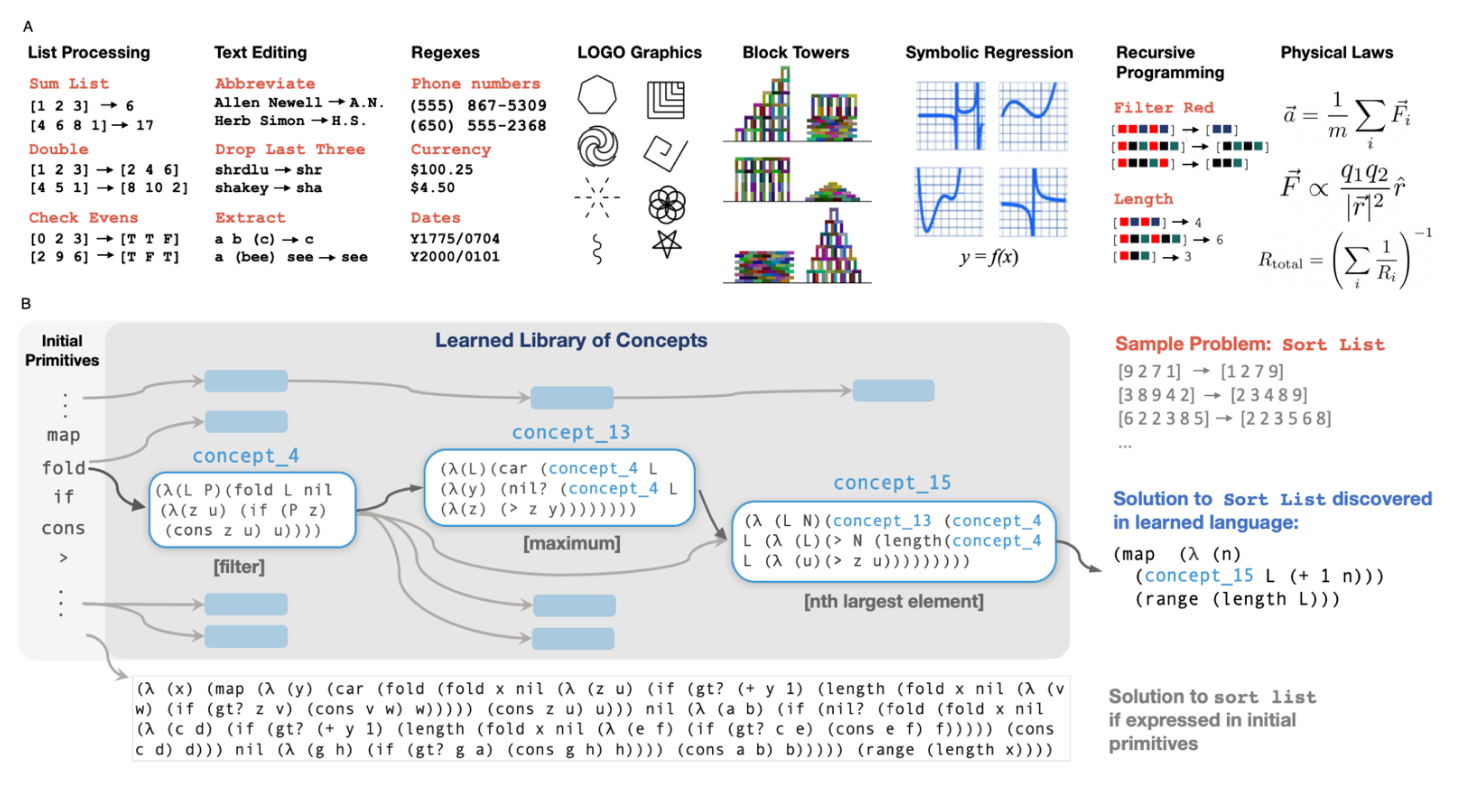
\includegraphics[width=\textwidth]{img/conc_library.png}
% \label{fig:conc_library}
% \caption{(A) 8 different domains of tasks. (B) Representation of the learned library of concepts. On the left we see the initial primitives from which the concepts in the middle region are composed. On the right we see a task as input-output relations and the found solution. On the bottom is the same solution expressed only with initial primitives. Image taken with permission from the original paper \cite{ellis_dreamcoder_2021}.}
% \end{figure*}

The model operates in three distinct phases. 

\paragraph{Wake} In the wake phase, the objective is to find the best program $\rho$  for each task $x \in X$ DreamCoder is presented with. Each task consist of one or a few (up to $\sim10$) examples. The system synthesises the programs using a neural network as the recognition model $Q$ to search through its library $D$.

\paragraph{Sleep: Abstraction} A key component of the success of DreamCoder is the refactoring of programs. In this phase, DreamCoder consolidates new abstractions from the programs it has found during the wake phase. Experiences are replayed, and commonalities between programs are found so that they can be abstracted into new concepts to use in the future. The objective is to find programs of minimum description length (MDL). 

\paragraph{Sleep: Dreaming} The objective during the dreaming phase is to train the recognition model $Q$ to perform MAP inference by both fantasies, and replays. When fantasising, programs are drawn from the learned library as a generative model. The model is then trained on the produced tasks. This ensures a large and varied data-set to learn from and encourages out-of-distribution generalisation. Replays, simply training on previously seen task-program pairs, ensures that the model improves its predictions on the actual tasks it needs to learn, by using its programs.

A Bayesian View
- What exactly happens?
- The generative model is a CFG, parameterized my a 
Include the parameterization of the generative model as a bigram transition matrix (three dimensional. Parent, arg index, depth?)





% “We use an EM algorithm to estimate the continuous parameters of the generative model, i.e. θ. Suppressing dependencies on D, the EM updates are θ = arg max θ log P (θ) + ∑ x Eqx [log P [ρ|θ]] (3) qx(ρ) ∝ P[x|ρ]P[ρ|θ]1 [ρ ∈ Bx] (4) In the M step of EM we will update θ by instead maximizing a lower bound on log P[ρ|θ], making our approach an instance of Generalized EM.” (from building hierarchical world models , one of the DreamCoder papers)



\begin{itemize}
    \item Frontier of primitives and abstracted concepts essentially form a markov blanket. 
\end{itemize}

\section{Transformer}

At the heart of the transformer is the self-attention mechanism, which enables the model to weigh the significance of different tokens in a sentence relative to a given token.

$$ \text{Attention}(Q, K, V) = \text{softmax}(\frac{QK^T}{\sqrt{d_k}})V $$
where
\begin{itemize}
    \item $Q$: Query matrix
    \item $K$: Key matrix 
    \item $V$: Value matrix
    \item $d_k$: Dimensions of keys
\end{itemize}

The self-attention mechanism allows the model to focus on different tokens with varying intensities, enabling it to capture long-range dependencies in the data.

Since the transformer lacks inherent notions of sequence order (unlike e.g. RNNs), positional encodings are added to the embeddings at the bottoms of the encoder and decoder stacks. This ensures that the model can attend to the position of words in the sequence. These encodings are added to the embeddings and have the same dimension, enabling the summed values to be processed in the self-attention layers.

Embeddings convert tokens into dense vectors of fixed size, capturing semantic meanings and relationships. This enables the model to understand relationships between different tokens.

\begin{itemize}
    \item Why is attention all you need?
    \item Why is the transformer architecture so relevant in the past few years?
    \item Why does it take away the need for archictecture search
    \item Multi-Head Attention: Instead of a single set of attention weights, the model uses multiple sets, enabling it to focus on different parts of the input for different tasks simultaneously.
    \item Feed-forward Networks: Each layer of the transformer contains a feed-forward neural network, which is applied independently to each position.
    \item Normalization and Residual Connections: These components help in stabilizing the activations and enabling deeper stacking of layers.
    \item Stephen Wolfram explains in his book about ChatGPT and the accompanying blog article how a thought can be seen as a trajectory through semantic space. 
\end{itemize}






%%%%%%%%% METHODS


Recent advancements in program synthesis have seen the rise of novel techniques aimed at generating code that not only satisfies a given specification but also matches human-written code patterns. One of the most notable methods in this sphere is DreamCoder. This model, along with several other state-of-the-art (SOTA) methodologies, has shown exceptional proficiency in understanding and generating complex code structures based on given specifications.

However, a critical examination of such methods, including DreamCoder, reveals a foundational limitation: their heavy reliance on syntactical constraints. While these constraints are undoubtedly vital for ensuring the correctness of generated programs, they do not necessarily guarantee a deep understanding or utilization of semantic relationships within the code. This is akin to learning the grammar of a language but missing out on the nuances and contexts that give meaning to words and phrases.

One could argue that the attention mechanism, as seen in transformers, provides a potential solution to this limitation. The attention mechanism inherently captures dependencies between various parts of an input, no matter how distant they might be. In the context of program synthesis, such a mechanism could be instrumental in deriving and maintaining meaningful semantic relationships between different code segments. The beauty of attention is that it provides a dynamic way to weigh different parts of the input based on context, potentially allowing a transformer-based model to capture intricate semantic details of a program.

Nevertheless, a transformer's capabilities come with its own set of challenges. While the attention mechanism offers a promising avenue for capturing semantic nuances, transformers, especially when trained from scratch, require colossal amounts of data to achieve satisfactory performance. The fundamental architecture of transformers necessitates this data-driven learning, often demanding diverse and extensive training datasets that might not always be available or feasible, especially in niche areas of program synthesis. Moreover, when the goal is to create a model of human cognitive abilities, it is obvious that humans do not have access to vast amounts of data, instead, we are able to infer causal relationships, from only a limited number of examples. E.g. consider the problem \texttt{[1,2,3] $\rightarrow$ [3,2,1]}. An astute reader might promptly conclude that the list has been reversed. 
Dougs analogies 

This is where GFlowNets (GFNs) carve their niche. Contrary to the data-hungry nature of transformers, GFNs do not necessitate gargantuan datasets for efficient training. Instead, they leverage a more intuitive approach: defining a reward distribution that's directly proportional to the objects (or programs) we intend to generate. This not only streamlines the learning process but also ensures that the synthesized programs are aligned with our desired outcomes.

In the realm of program synthesis, our objectives are clearly defined. We aim to construct objects, or more specifically, pieces of code that precisely meet the given specification. This isn't just about producing syntactically correct code; it's about generating semantically rich and efficient programs that can effectively solve the specified problem without superfluous or redundant components.







\begin{itemize}
    \item What is the problem? why can't we marginalise over the CFG? or can we? 
    \item How does GFN or DC deal with it? 
\end{itemize}


